\documentclass[12pt]{article}
\usepackage[utf8]{inputenc}
\usepackage[T2A]{fontenc}
\usepackage[russian]{babel}
\usepackage{amsmath}
\usepackage{amssymb}
\usepackage{dsfont}
\usepackage[dvipsnames]{xcolor}
\usepackage{setspace}
\usepackage{multirow}
\usepackage[a4paper, outer=1.5cm, inner=1.5cm, top=1cm, bottom=1cm]{geometry}
\usepackage{graphicx}
\usepackage{skull}
\usepackage{wasysym}
\usepackage{float}
\graphicspath{{.images/}}
\usepackage{hyperref}
\hypersetup{colorlinks=true, linkcolor=blue, filecolor=magenta, urlcolor=cyan}
\usepackage[firstpage]{draftwatermark}
\SetWatermarkText{
    $\qquad\qquad\qquad\qquad\qquad$\parbox{7cm}{\begin{center}
    
\includegraphics[width = 0.08\textwidth]{lion-logo.png}\bigskip\\~\bigskip\\~\vspace{-24mm}\\~\end{center}}
}
\SetWatermarkAngle{0}
\SetWatermarkScale{1.5}
\usepackage{etoolbox}

\newtoggle{ifsolved}
\newtoggle{needhelp}
\newcounter{num}
\setcounter{num}{1}

\newcommand{\newnum}{\par\textbf{\textnumero\arabic{num}}\stepcounter{num}}
\newcommand{\sol}{\vspace{3mm}\par\textbf{Решение: }}
\newcommand{\ans}{\vspace{3mm}\par\textbf{Ответ: }}
\newcommand{\hint}{\vspace{3mm}\par\textbf{Подсказка: }}
\newcommand{\mode}[1]{
\ifstrequal{#1}{0}{\togglefalse{ifsolved}\togglefalse{needhelp}}{\ifstrequal{#1}{1}{\togglefalse{ifsolved}\toggletrue{needhelp}}{\ifstrequal{#1}{2}{\toggletrue{ifsolved}\togglefalse{needhelp}}{\toggletrue{ifsolved}\toggletrue{needhelp}}}}} %if 0 - if 1 - if 2 - else
%\newenvironment{problem}[8]{%#1, #2, #3
%\parbox{\linewidth}{\vspace{4mm}\ifstrequal{#4}{(лёгкая)}{\newnum\textbf{.}}{\newnum\textbf{*.} } \\ #5}
%\iftoggle{ifsolved}{\sol #6}{}
%\iftoggle{ifsolved}{\ans #7}{}
%\iftoggle{needhelp}{\hint #8}{}}

\newenvironment{problem}[8]{%#1, #2, #3
\parbox{\linewidth}{\vspace{5mm}\ifstrequal{#4}{(лёгкая)}{\newnum\textbf{.}}{\newnum\textbf{*.} } \\ #5}
\iftoggle{ifsolved}{\sol #6}{}

\iftoggle{ifsolved}{\parbox{\linewidth}{\ans #7}}{}
\iftoggle{needhelp}{\parbox{\linewidth}{\hint #8}}{}}

\newenvironment{mylist} %custom list
{ \begin{itemize}
    \setlength{\itemsep}{0pt}
    \setlength{\parskip}{0pt}
    \setlength{\parsep}{0pt}     }
{ \end{itemize}                  }

\newenvironment{homeass}[1]{\vspace*{-1.5cm}
\iftoggle{ifsolved}{
    \section*{\center{Решение домашнего задания к #1.}}
}{
    \section*{\center{\textcolor{Sepia}{Домашнее задание к #1}}}
} \vspace{7mm}\large}

\parindent=0pt
\pagestyle{empty}
%$\!$[\arabic{class}.\arabic{num}]
%\ifnumcomp{\value{counter}}{>}{1}{true}{false}
%\definecolor{Gray}{gray}{0.9}
%\definecolor{mypink}{RGB}{219, 48, 122}
%\newcolumntype{g}{>{\columncolor{Gray}}p{2.8cm}}

\begin{document}
\large
\mode{7}
%0 for problems without hints
%1 for problems + hints
%2 for problems + solutions + answers
%else: show all

{\centering\section*{СПИСОК ЗАДАЧ}}

{\centering\subsection*{\smallskip\\\textcolor{green}{\textbf{Полезные вещи, которые можно и нужно копипастить:}}}}

\subsection*{\textcolor{Emerald}{\textbf{Полезные шпаргалки по LaTeXу:}}}

\textbf{Пример вставки рисунка:}

\begin{minipage}{\linewidth}
    \begin{minipage}{0.54\linewidth}
    см. рисунок справа\\
    Текст к собственно пикче, примерно всегда это либо развёрнутое описание, либо большая часть решения задачи --- стремимся экономить пространство, если это можно сделать.
    \end{minipage}
    \hspace{0.05\linewidth}
    \begin{minipage}{0.4\linewidth}
    \begin{figure}[H] 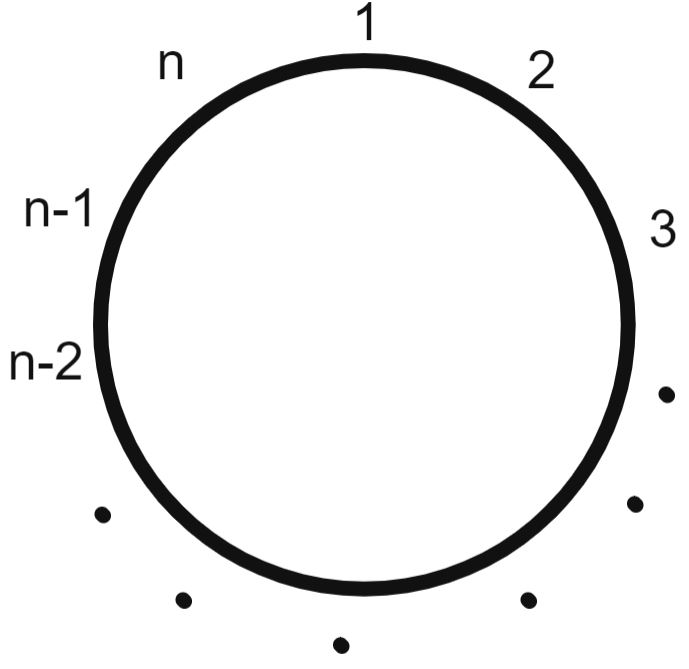
\includegraphics[width=\linewidth]{sol3} %тут поменять имя пикчи
    \end{figure}
    \end{minipage}
\end{minipage}

\textbf{Дефолтные математические знаки и символы:}\\
$\geqslant$,
$\leqslant$,
$a^{b}$,
$x_{i}$,
$\sqrt{a}$,
$\frac{a}{b}$,
$\displaystyle \frac{a}{b}$,
$\cdot$
$\;\Rightarrow\;$,
$\;\Leftrightarrow\;$,
$1{,}2$.
О промежутках:
$a\!b$,
$a\,b$,
$a\:b$,
$a\;b$,
$a\quad b$.

\textbf{Стандартные система и совокупность уравнений / неравенств:}\\
$\left\{
\begin{aligned}
f(x) &= 0 \\
g(x) &= 1
\end{aligned}\right.$

$\left[\begin{aligned}
&\left\{\begin{aligned}
f(x) &\geqslant a \\
g(x) &= b
\end{aligned}\right.\\
&\left\{\begin{aligned}
f(x) &< a \\
g(x) &= -b
\end{aligned}\right.
\end{aligned}\right.$

\subsection*{\textcolor{Emerald}{\textbf{Не математическое, но полезное:}}}
% комментарий в любом месте документа, который нигде не будет видно. Можно использовать для написания заметок-вопросов по задачам
\textbf{Пример таблицы:}

\begin{tabular}{|c|c|c|}
\hline
    $a$ & $b$ & текст
\\\hline
    $c$ & $d$ & мораль
\\\hline
\end{tabular}\\

\textbf{Отступы:} между\smallskip\\ строками\medskip\\ \textbf{Тире} --- это три дефиса.\\
\textbf{Списки:}
\begin{mylist}
\item [$\bullet$] это был пункт а
\item [2)] а это уже пункт номер 2 с изменённым заголовком
\end{mylist}

\subsection*{\textcolor{Emerald}{\textbf{Всё, неупомянутое выше (или если просто что-то не так):}}}
\begin{mylist}
\item [$\bullet$] Решение отдельных вопросов касательно ТеХа нужно искать в \href{https://www.mccme.ru/free-books/llang/newllang.pdf}{Львовском}.

\item [$\bullet$] Найти произвольный символ, который нужен, можно в \href{http://detexify.kirelabs.org/classify.html}{Detexify}.

\item [$\bullet$] Если возникли сомнения при решении, ответ практически ко всем задачам можно проверить с помощью \href{https://www.wolframalpha.com/}{WolframAlpha}.

\item [$\bullet$] Если в задаче нужно создать картинку, то лучше пока отложить эту задачу. Все графики планируется централизованно нарисовать (или перерисовать) в геогебре.

\item [\textcolor{brown}{\textbf{!!}}] Важно ставить \textcolor{red}{\textbf{$\spadesuit$}}
(или просто red) в тело задачи в случае серьёзных вопросов к решению и какой-то вопиющей лажи.

\item [\textcolor{brown}{\textbf{!!}}] Важно ставить \textcolor{olive}{\textbf{$\spadesuit$}}
(или просто olive) в тело задачи в случае не самого удачного текста и кривых отступов.
\end{mylist}

\subsection*{\textcolor{Violet}{\textbf{Комментарии:}}}% а также невидимые комментарии - так можно оставлять заметки-вопросы прямо в задаче, чтобы потом было понятно, в чём вопрос.
\begin{mylist}
\item [$\skull$] Переставлять задачи местами --- очень плохая идея.

\item [$\smiley$] При двойном клике по тексту pdf справа происходит автоматический переход к этому месту в латех-коде, а для обратного перехода можно нажать стрелку вправо (висит сверху между pdf и латех-кодом).

\item [$\smiley$] Если есть размышления, дописывать red/olive к задаче или не дописывать, то лучше всё-таки дописать.

\item [$\skull$] Самое плохое, что можно сделать --- написать в любое поле из трёх (НаписанноеРешение/ВерныйОтвет/Подсказка) только половину того, что надо, никак это не отметить, и потом пойти дальше.\\ Нужно в этот момент писать red/olive в случайном месте задачи, чтобы потом вычислить это с помощью Ctrl+F по всему документу (и это то, что потом будет делаться долго и тщательно)
\end{mylist}

\newpage
\setcounter{num}{1}


\hypertarget{6.1}{{\centering\section*{\bigskip\\\textcolor{Blue}{\hyperlink{start2}{\textcolor{Blue}{6.1}} Делимость-1.}\vspace{-5mm}}}}

\begin{problem}{Делители и кратные.}{6.1.1}{6K \textcolor{olive}{\textbf{$\spadesuit$}}}{(лёгкая)}
{Сколько существует чисел от $1$ до $41$, которые делятся на $7$, но не делятся на $2$?}
{Выпишем те числа, которые делятся на 7: это 7, 14, 21, 28, 35 (следующее число~--- 42~--- уже больше 41). Выберем из них те, которые не делятся на 2, то есть нечётные. Остаются 7, 21, 35: 14 и 28~--- чётные.}
{Таких чисел три: это 7, 21 и 35.}{Для начала, а сколько всего чисел, которые делятся на 7?}
\end{problem}

\begin{problem}{Признаки делимости на 2, 5, 10, 100.}{6.1.2}{6S \textcolor{olive}{\textbf{$\spadesuit$}}}{(лёгкая)}
{Какой цифрой оканчивается произведение первых девяти натуральных чисел?}
{Среди первых девяти натуральных чисел есть 5 и 2. Их произведение оканчивается на 0, а значит и произведение всех девяти чисел оканчивается на 0.

}
{На 0.}{Какой признак делимости на 10?}
\end{problem}

\begin{problem}{Признаки делимости на 2, 5, 10, 100.}{6.1.2}{6K}{(лёгкая)}
{Делится ли значение выражения $11 \cdot 21 \cdot 31 \cdot 41 \cdot 51 - 111$ на 10 нацело?}
{Число $11 \cdot 21 \cdot 31 \cdot 41 \cdot 51$ оканчивается на 1 (так как при умножении чисел в столбик последней всегда будет единица). После вычитания 111 последней цифрой станет 0, а значит число будет делиться на 10 нацело.}
{Да, это выражение делится на 10 нацело.}{Какова последняя цифра числа $11 \cdot 21 \cdot 31 \cdot 41 \cdot 51$?}
\end{problem}

\begin{problem}{Признаки делимости на 2, 5, 10, 100.}{6.1.2}{6K}{*}
{Напиши все трёхзначные числа, записанные цифрами 1, 2, 5 (без повторений).
\\1) Сколько всего таких чисел?\\
2) Сколько из них делится на 2?\\
3) Сколько из них делится на 5?\\
4) Найди сумму всех этих чисел и проверь, делится ли эта сумма на 111.\\
5) Делится ли сумма всех шести чисел на 111, если выбрать какие-то другие три цифры (не 1, 2, 5)?}
{1) Таких чисел шесть: это числа 125, 152, 215, 251, 512, 521.\smallskip\\
2) На 2 делятся только те числа, которые оканчиваются на чётную цифру~--- в нашем случае таких чисел только два, это $152$ и $512$.\smallskip\\
3) На 5 делятся только те числа, которые оканчиваются на 5 или 0. Поэтому таких чисел тоже два: это 125 и 215.\smallskip\\
4) Вычислим сумму всех чисел: $125 + 152 + 215 + 251 + 512 + 521 = 277 + 466 + 1033 = 743 + 1033 = 1776$. Эта сумма делится на 111: $1776 = 1110 + 666 = 16 \cdot 111$.\smallskip\\
5) Допустим, выбрали какие-то три цифры $a$, $b$, $c$. Тогда из них получатся шесть чисел $\overline{abc}$, $\overline{acb}$, $\overline{bac}$, $\overline{bca}$, $\overline{cab}$, $\overline{cba}$ (здесь чёрточка над числом ставится для того, чтобы напомнить, что это единое трёхзначное число, а не произведение $a$, $b$ и $c$).\\
Используем хитрость и перепишем числа как сумму сотен, десятков, и единиц:\\
$\overline{abc} = 100a + 10b + c$, \hfill
$\overline{bac} = 100b + 10a + c$, \hfill
$\overline{cab} = 100c + 10a + b$,\\
$\overline{acb} = 100a + 10c + b$, \hfill $\overline{bca} = 100b + 10c + a$, \hfill $\overline{cba} = 100c + 10b + a$.\\
Сложим всё, получается $200a + 200b + 200c + 20a + 20b + 20c + 2a + 2b + 2c$, или, что то же самое, $200 \cdot (a + b + c) + 20 \cdot (a + b + c) + 2 \cdot (a + b + c) = 222 \cdot (a + b + c)$.\\
Данное выражение, разумеется, всегда делится на 111 ($222 = 2 \cdot 111$).\\
Таким образом, сумма всех возможных чисел, собранных из трёх произвольных заранее выбранных цифр без повторений, всегда делится на 111.}
{Сумма этих шести чисел всегда делится 111, какие бы цифры мы не взяли.

}{Для решения последнего пункта надо отдельно посчитать сумму числа сотен, числа десятков, и числа единиц.}
\end{problem}

\begin{problem}{Признаки делимости на 2, 5, 10, 100.}{6.1.2}{6K}{(лёгкая)}
{Рассмотрим все числа $\alpha$, для которых произведение $44 \cdot \alpha$ заканчивается на $0$.\\ Сколько среди таких чисел $\alpha$ двузначных?}
{Число будет заканчиваться на 0 тогда и только тогда, когда оно \\делится на 5 и на 2 одновременно. Число $44 \cdot \alpha$ уже точно делится на 2. Это значит, что 5 должна быть в $\alpha$ (то есть $\alpha$ делится на 5). Выясним, сколько двузначных чисел делятся на 5: 10, 15, 20, 25, 30, 35, 40, 45, 50, 55, 60, 65, 70, 75, 80, 85, 90, 95. 100 уже трёхзначное. Значит, таких чисел всего 18 (и все они перечислены выше).

}
{Двузначных чисел 18 штук, они перечислены выше.}{Число оканчивается на 0, если оно делится на 10.\\ Какой признак делимости на 10?}
\end{problem}

\begin{problem}{Признаки делимости на 2, 5, 10, 100.}{6.1.2}{6K}{*}
{Сколькими нулями оканчивается произведение $1 \cdot 2 \cdot 3 \cdot 4 \cdot \ldots \cdot 1533 \cdot 1534 \cdot 1535$?}
{Количество нулей равно $N$, где $N$~--- сколько раз можно поделить это число на 10 нацело, количество десяток. Каждая десятка~--- это $2 \cdot 5$, то есть то ли двоек, то ли пятерок в этом числе ровно $N$ штук. Более того, понятно, что речь идёт именно о пятерках: ведь в этом числе двоек больше, чем пятерок, а число десяток определяется тем из множителей 2 и 5, которого меньше чем другого.\smallskip\\
Таким образом, нужно посчитать, сколько пятёрок есть в числе $1 \cdot 2 \cdot 3 \cdot 4 \cdot \ldots \cdot 1533 \cdot 1534 \cdot 1535$. Тут, однако, таится подвох, который можно не заметить.\\ Во-первых, конечно же, каждый пятый множитель из этих 1535 делится на 5, то есть таких всего $1535 : 5 =$ \textbf{307}, и мы уже насчитали 307 пятёрок.\smallskip\\ Но ведь каждое пятое число из делящихся на 5 будет делиться уже на 25, то есть пятёрок где-то будет две... Найдём количество чисел, среди которых есть вторая пятёрка: таких будет 61, поскольку $307 : 5 =$ \textbf{61} (ост. 2).\smallskip\\
А ведь может быть и третья пятёрка (в числах 125, 250, 375, 500, $\ldots$).
Таких чисел будет 12 (как и раньше, их в 5 раз меньше, чем предыдущих: $61 : 5 =$ \textbf{12} (ост. 1). Вот они все подряд: 125, 250, 375, 500, 625, 750, 875, 1000, 1125, 1250, 1375, 1500.\smallskip\\
Четвёртая пятёрка: таких чисел два ($12 : 5 =$ \textbf{2} (ост. 2)). Это числа 625 и 1250.\smallskip\\
Пятой пятёрки ни в одном множителе не будет ($2 : 5 =$ \textbf{0} (ост. 2))\smallskip\\
Итого, всего пятёрок: $307 + 61 + 12 + 2 + 0 = 368 + 14 = 382$ штуки. Так как двоек в этом числе точно больше 382, то десяток всего образуется ровно 382.\\ Значит, данное число оканчивается на 382 нуля.}
{Это число оканчивается на 382 нуля.\\
\textit{Замечание:} для таких чисел (произведения натуральных чисел от 1 до $n$) есть сокращённая форма записи $n!$ (читается <<эн факториал>>, от латинского factor~--- множитель). То есть $1 \cdot 2 \cdot \ldots \cdot 1534 \cdot 1535 = 1535!$, а например $4! = 1 \cdot 2 \cdot 3 \cdot 4 = 24$.}{Нужно подсчитать, сколько раз 5 входит в это число как множитель. Однако при подсчёте надо иметь в виду, что есть такие числа, как 25, 50, 125, где пятёрок больше одной.}
\end{problem}

\begin{problem}{Признаки делимости на 2, 5, 10, 100.}{6.1.2}{6K}{*}
{Доказать, что сумма двух последовательных нечётных чисел делится на 4.}
{Пусть $n$~--- какое-то нечётное число. Тогда следующее за ним нечётное число равно $n + 2$, а сумма этих двух чисел равна $n + n + 2 = 2n + 2 = 2 \cdot (n + 1)$.\\ $n + 1$ является чётным числом, поскольку $n$ нечётно. Значит сумма двух нечётных чисел равна $2 \,\times\!$ чётное число, то есть делится на 4. Доказано.\smallskip\\
Есть и другой способ доказательства: рассмотрим числа 1 и 3. Их сумма равна 4 и делится на 4. Сумма следующей пары~--- 3 и 5 отличается от предыдущей на 4: $3 + 5 = (1 + 4) + 3 = (1 + 3) + 4$. Следующая пара, 5 и 7, также отличается на 4: $5 + 7 = (5 + 3) + 4$, и так далее. Таким образом, полученная сумма всегда равна какому-то количеству четвёрок и следовательно всегда делится на 4.}
{Смотри доказательство выше.}{Пусть $n$~--- нечётное число. Чему тогда равна сумма чисел?}
\end{problem}

\begin{problem}{Признаки делимости на 3 и на 9.}{6.1.3}{6K}{(лёгкая)}
{Дима написал число гугол (единица со ста нулями) и вычел из него $100$.\\ Найти сумму цифр того числа, которое получилось в итоге.}
{После вычитания получится 100-значное число, кончающееся на два нуля: $\underbrace{9999...999}_{98 \text{ девяток}}\!00$. Сумма его цифр равна $9 \cdot 98 = 810 + 72 = 882$.}
{Сумма цифр этого числа равна 882.}{Получившееся число будет 100-значным.}
\end{problem}

\begin{problem}{Признаки делимости на 3 и на 9.}{6.1.3}{6K}{(лёгкая)}
{Замени в записи числа $152{**}$ звёздочки таким образом, чтобы получившееся пятизначное число делилось на $6$. Запиши все возможные варианты.}
{Число делится на 6 если и только если оно делится и на 2 и на 3. Поэтому последней цифрой может быть только чётная, что даёт нам 5 вариантов:\\ $152{*}0$, $152{*}2$, $152{*}4$, $152{*}6$, $152{*}8$. Пусть оставшаяся цифра равна $x$.\\
Так как число должно делиться на 3, сумма его цифр должна делиться на 3. Рассмотрим все варианты отдельно:\smallskip\\
1) $152{*}0 \;\Rightarrow\; 1 + 5 + 2 + x + 0 = 8 + x$ должно делиться на 3 $\Rightarrow\; x = 1$; 4; 7.\\
Получилось 3 подходящих числа: 15210, 15240 и 15270.\smallskip\\
2) $152{*}2 \;\Rightarrow\; 8 + x + 2 = 10 + x$ должно делиться на 3 $\Rightarrow\; x = 2$; 5; 8.\\
Получилось 3 подходящих числа: 15222, 15252 и 15282.\smallskip\\
3) $152{*}4 \;\Rightarrow\; 8 + x + 4 = 12 + x$ должно делиться на 3 $\Rightarrow\; x = 0$; 3; 6; 9.\\
Получилось 4 подходящих числа: 15204, 15234, 15264 и 15294.\smallskip\\
4) $152{*}6 \;\Rightarrow\; 8 + x + 6 = 14 + x$ должно делиться на 3 $\Rightarrow\; x = 1$; 4; 7.\\
Получилось 3 подходящих числа: 15216, 15246 и 15276.\smallskip\\
5) $152{*}8 \;\Rightarrow\; 8 + x + 8 = 16 + x$ должно делиться на 3 $\Rightarrow\; x = 2$; 5; 8.\\
Получилось 3 подходящих числа: 15228, 15258 и 15288.\smallskip\\
Итого, всего получилось 16 подходящих чисел: 15204, 15210, 15216, 15222, 15228, 15234, 15240, 15246, 15252, 15258, 15264, 15270, 15276, 15282, 15288, 15294.\smallskip\\
\textit{Альтернативный способ решения: }заметить, что число 15204 подходит, а дальше прибавлять по 6 до тех пор, пока число не станет слишком большим.}
{Всего получилось 16 подходящих чисел: 15204, 15210, 15216, 15222, 15228, 15234, 15240, 15246, 15252, 15258, 15264, 15270, 15276, 15282, 15288, 15294.}{Какой признак делимости на 6?}
\end{problem}

\begin{problem}{Признаки делимости на 3 и на 9.}{6.1.3}{6K}{(лёгкая)}
{На некоторой олимпиаде все задачи оцениваются либо в $2$, либо в $3$ балла~--- $10$ задач по $2$ балла и $10$ задач по $3$ балла. Какое наименьшее возможное количество «$2$-балльных» задач мог верно решить участник, набравший в сумме $37$ баллов?}
{Пусть участник решил $n$ 3-балльных задач и не решил ни одной 2-балльной задачи. Тогда $3 \cdot n = 37$. Но $37$ не делится на 3 (сумма цифр равна 10), поэтому такое невозможно. Хорошо, допустим одна 2-балльная задача была решена. Тогда $37 = 2 + 3 \cdot n \;\Rightarrow\; 35 = 3 \cdot n$. Но 35 тоже не делится на 3, поэтому участник решил более чем одну 2-балльную задачу. Проверим, могло ли быть две задачи: в этом случае $37 = 2 \cdot 2 + 3 \cdot n \;\Rightarrow\; 33 = 3 \cdot n \;\Rightarrow\; n = 11$.\\ То есть участник мог решить две 2-балльных и одиннадцать 3-балльных задач, и получить в сумме 37 баллов.\\ Следовательно, наименьшее количество решённых 2-балльных задач~--- две.}
{Этот участник решил верно как минимум две двухбалльных задачи.}{Эту задачу можно решить умным перебором.}
\end{problem}

\begin{problem}{Признаки делимости на 3 и на 9.}{6.1.3}{6S}{(лёгкая)}
{Поставь в записи числа 4$\ast$651 вместо $\ast$ такую цифру, чтобы получилось число, которое при делении на 3 даёт в остатке 1.}
{Если это число при делении на 3 даёт в остатке 1, то это значит, что число $4{\ast}650$ делится на 3 нацело. Используем признак делимости на 3: число делится на 3 тогда и только тогда, когда его сумма цифр делится на 3.\\ Сумма цифр этого числа равна $4 + x + 6 + 5 + 0 = 15 + x$, откуда $x = 0$, $x = 3$, $x = 6$, $x = 9$~--- подходящие варианты.\\ Следовательно, любое из чисел $40651$, $43651$, $46651$, $49651$ подходит.}
{Есть четыре подходящих варианта: $40651$, $43651$, $46651$, $49651$.}{Какой признак делимости на 3? Есть несколько подходящих ответов.}
\end{problem}

\begin{problem}{Признаки делимости на 3 и на 9.}{6.1.3}{6S}{(лёгкая)}
{В числе $7030506$ замени все нули одной и той же цифрой так, чтобы полученное число делилось на 9.}
{После того, как все нули будут заменены одной и той же цифрой $a$, получится число $7a3a5a6$. Используем признак делимости на 9: число делится на 9 тогда и только тогда, когда его сумма цифр делится на 9.\\ Сумма цифр нашего числа равна $7 + a + 3 + a + 5 + a + 6 = 21 + 3a$.\\ Значит, сумма цифр числа будет делиться на 9, если $a = 2$ ($21 + 6 = 27$), $a = 5$ ($21 + 15 = 36$), или $a = 8$ ($21 + 24 = 45$). Других вариантов нет.\\ Таким образом, есть три подходящих варианта: 7232526, 7535556 и 7838586.}
{Подходят числа 7232526, 7535556 и 7838586}{Какой признак делимости на 9? Есть несколько подходящих ответов.}
\end{problem}

\begin{problem}{Признаки делимости на 3 и на 9.}{6.1.3}{6S}{(лёгкая)}
{Найди наибольшее пятизначное число, которое делится на 2 и на 3.}
{Число делится на 2 и на 3, если оно кончается на чётную цифру, а его сумма цифр делится на 3. Рассмотрим самые большие пятизначные числа, кончающиеся на чётные цифры: это 99990, 99992, 99994, 99996, 99998. Выясним, которые из них делятся ещё и на 3: сумма цифр чисел 99990 и 99996 делится на 3, а остальных~--- нет. Таким образом, 99996~--- самое большое пятизначное число, которое делится и на 2, и на 3 (следующее число 100002 уже шестизначное).}
{99996.}{Числа, которые делятся и на 2, и на 3~--- числа, делящиеся на 6.}
\end{problem}

\begin{problem}{Признаки делимости на 3 и на 9.}{6.1.3}{6S}{(лёгкая)}
{Восстановить запись, не вычисляя: $14 \cdot 15 \cdot 16 \cdot 17 \cdot 18 \cdot 19 = 1953?040$.}
{Можно заметить, что среди множителей слева есть число 18, которое делится на 9. Тогда произведение этих чисел делится на 9, а значит выполнен признак делимости на 9: $\,1 + 9 + 5 + 3 + {?} + 0 + 4 + 0 = 22 + {?}$ делится на 9.\\
Раз число $22 + {?}$ делится на 9, то пропущенной цифрой может быть только 5 (тогда сумма цифр будет равна 27).}
{$14 \cdot 15 \cdot 16 \cdot 17 \cdot 18 \cdot 19 = 19535040$.}{Покажи, что это число делится на 9.}
\end{problem}

\begin{problem}{Признаки делимости на 3 и на 9.}{6.1.3}{6S}{(лёгкая)}
{К числу 37 припиши слева и справа одну и ту же цифру так, чтобы полученное число делилось на 6.}
{Пусть была приписана цифра $c$. Тогда получится четырёхзначное число $\overline{c37c}$. Число делится на 6, если оно делится и на 2, и на 3.\\
Из признака делимости на 2 получаем, что $c = 0 / 2 / 4 / 6 / 8$.\\
Из признака делимости на 3 получаем условие на сумму цифр: $10 + 2c \;\vdots\; 3$, откуда $c = 1 / 4 / 7$. Поскольку должны быть одновременно выполнены оба условия, $c = 4$. Получается число 4374, надо приписать четвёрку.}
{4374.}{Какой признак делимости на 6?}
\end{problem}

\begin{problem}{Признаки делимости на 3 и на 9.}{6.1.3}{6S}{(лёгкая)}
{Найди четырёхзначное число, которое делится на 4, а при делении на 3 даёт остаток 2.}
{Самое простое четырёхзначное число, которое делится на 4~--- это 1000. Оно, однако, при делении на 3 даёт остаток 1 (остаток при делении числа на 3 всегда равен остатку при делении его суммы цифр на 3).\\
Следующее число, которое делится на 4~--- 1004. Оно равно $1002 + 2$, и даёт при делении на 3 в остатке 2. Разумеется, подходят и многие другие числа.}
{Например, число 1004. А вообще, любое число вида $1004 + 12 \cdot k$, где $k$~--- натуральное число (1016, 1028, 1040, $\ldots$), также подойдёт.}{Таких чисел много~--- достаточно выбрать любое подходящее.}
\end{problem}

\begin{problem}{Признаки делимости на 3 и на 9.}{6.1.3}{6S red в НОК его}{(лёгкая)}
{Фермер привёз на базар огурцы. Когда он стал считать их десятками, то не хватило двух огурцов до полного числа десятков.\\ Когда он стал считать огурцы дюжинами, то осталось 8 огурцов.\\ Сколько огурцов привёз фермер, если их было больше 300, но меньше 400?}
{Поскольку до полного числа десятков не хватило двух огурцов, это значит, что количество огурцов~--- трёхзначное число~--- заканчивается на 8.\\ С другой стороны, получается, что без этих восьми огурцов огурцов будет целое число дюжин, то есть нужно найти число, которое делится и на 10, и на 12.\\ Если число делится и на 10, и на 12, то оно делится на 60 (Нашли НОК).\\ Выписываем числа, делящиеся на 60: 60, 120, 180, 240, 300, 360, 420,$\ldots$\\ Так как огурцов было от 300 до 400, остаются только два варианта~--- 300 и 360, и соответственно 308 или 368 огурцов.}
{Фермер привёз не то 308, не то 368 огурцов~--- точнее определить нельзя.}{Осторожно, тут два возможных правильных варианта ответа!}
\end{problem}

\begin{problem}{Признаки делимости на 3 и на 9.}{6.1.3}{6S}{*}
{К числу 10 припиши слева и справа по одной цифре так, чтобы полученное число делилось на 72.}
{Число будет делиться на 72, если оно делится на 8 и на 9.\\ Признак делимости на 8: последние три цифры числа делятся на 8, то есть $\overline{10y}$ делится на 8, а значит, это число 104 и последняя цифра этого числа равна 4.\\ Теперь разберёмся с первой цифрой. Нам известно, что число $\overline{x104}$ делится на 9, а значит, его сумма цифр делится на 9. Но его сумма цифр равна $x + 5$, откуда $x = 4$, остальные варианты не подходят. Получается, что это число 4104.}
{Это число 4104, других вариантов нет.}{На что обязано делиться число, если оно делится на 72?}
\end{problem}

\begin{problem}{Признаки делимости на 3 и на 9.}{6.1.3}{6S}{*}
{Найти цифры числа 42$\ast$4$\ast$, если известно, что это число делится на 72.}
{Число будет делиться на 72, если оно делится на 8 и на 9.\\ Пусть $a$~--- первая цифра, а $b$~--- вторая. Раз это число делится на 9, то по признаку делимости на 9, сумма цифр $4 + 2 + a + 4 + b = 10 + a + b$ должна делиться на 9, откуда $a + b = 8$ или $a + b = 17$.\vspace{-3mm}\\
Это даёт следующие варианты $a$ и $b$: $\;\;\;$ \begin{tabular}{|c|c|c|c|c|c|c|c|c|c|c|c|}
\hline
    $a$: & 0 & 1 & 2 & 3 & 4 & 5 & 6 & 7 & 8 & 8 & 9\\
    $b$: & 8 & 7 & 6 & 5 & 4 & 3 & 2 & 1 & 0 & 9 & 8\\
    \hline
\end{tabular}\smallskip\\
Теперь используем признак делимости на 8: для начала отбросим все варианты с нечётным $b$~--- они точно не могут делиться на 8. Остаются числа 42048, 42246, 42444, 42642, 42840, 42948. Найдём среди них те, которые делятся на 8 (то есть те, у которых последние три цифры делятся на 8). 42048 подходит, 42246~--- нет ($246 = 240 + 6$), 42444~--- тоже нет ($444 = 400 + 44$), 42642~--- нет ($642 = 640 + 2$), 42840~--- подходит, 42948~--- нет ($948 = 960 - 12$). Итого, либо это 42048, либо 42840.

}
{Пропущенные цифры числа~--- 0 и 8. Оба числа 42048 и 42840 подходят.}{На что обязано делиться число, если оно делится на 72?\\ Сделать перебор оставшихся вариантов.}
\end{problem}

\begin{problem}{Признаки делимости на 3 и на 9.}{6.1.3}{6S}{(лёгкая)}
{Найди цифры числа 72$\ast$3$\ast$, если известно, что это число делится на 45.}
{Если число делится на 45, то оно делится на 5 и на 9. Следовательно, последняя цифра числа~--- либо 5, либо 0. Рассмотрим каждый пример отдельно:\\ В первом случае, если на конце стоит цифра 5, то число 72$\ast$35 делится на 9, а значит его сумма цифр делится на 9. $7 + 2 + {\ast} + 3 + 5 = 17 + {\ast}$, откуда вторая пропущенная цифра равна 1 и получается число 72135.\\ Во втором случае, если на конце стоит 0, то у числа 72$\ast$30 сумма цифр равна $12 + {\ast}$, откуда по признаку делимости на 9 мы получаем, что пропущена цифра 6 и это число 72630. $\;$ Итого, это 72135 или 72630.}
{Это число~--- 72135 или 72630.}{На что обязано делиться число, если оно делится на 45?\\ Осторожно, тут возможны два варианта ответа.}
\end{problem}

\begin{problem}{Признаки делимости на 3 и на 9.}{6.1.3}{6S}{*}
{Какие цифры надо поставить вместо <<?>>, чтобы число 517?? делилось на 6, 7 и 9 одновременно?}
{Если число делится на 6, оно обязано быть чётным, поэтому последняя цифра обязательно чётная. Если число делится на 9, сумма его цифр делится на 9. Так как сумма известных нам трёх цифр равна 13, сумма двух неизвестных цифр равна или 5, или 14. В итоге получаются возможными следующие 5 вариантов:\\
51750, 51732, 51714, 51786, 51768. Проверим каждое число на делимость на 7:\smallskip\\
$51750 = 49000 + 2100 + 630 + 20 \;\Rightarrow\;$ не подходит\\
$51732 = 49000 + 2100 + 630 + 2\;\, \;\Rightarrow\;$ не подходит\\
$51714 = 49000 + 2100 + 560 + 54 \;\Rightarrow\;$ не подходит\\
$51786 = 49000 + 2100 + 630 + 56 \;\Rightarrow\;$ подходит\\
$51768 = 49000 + 2100 + 630 + 38 \;\Rightarrow\;$ не подходит.}
{Нужно поставить цифры 8 и 6: всем условиям удовлетворяет число 51786.

}{Делимость на 7 лучше оставить на конец решения, а для начала стоит проверить все остальные признаки делимости и оставить только 5 подходящих чисел-кандидатов.}
\end{problem}

\begin{problem}{Признаки делимости на 3 и на 9.}{6.1.3}{6K}{(лёгкая)}
{В числе $32{*}7{*}$ замени звёздочки на цифры таким образом, чтобы получившееся пятизначное число делилось на $12$. Найди все варианты.\\ Сколько из них делится на $36$?}
{Если число делится на 12, это тоже самое, что и если число делится и на 3, и на 4 одновременно. Признак делимости на 4: число делится на 4, если две его последние цифры делятся на 4. Вследствие этого получаем, что последняя цифра~--- 2 или 6. Рассмотрим первый случай, если это число $32{*}72$.\\ Тогда согласно признаку делимости на 3, сумма цифр должна делиться на 3, а она равна $14 + {*}$. Таким образом, пропущенная цифра в этом случае~--- 1/4/7.\\
Второй случай: если число~--- $32{*}76$, то сумма его цифр равна $18 + {*}$.\\ Тогда для пропущенной цифры есть целых 4 варианта: 0/3/6/9.\\
Итого, таких чисел 7: $\;$32172, 32472, 32772, 32076, 32376, 32676, 32976.\smallskip\\ Для того чтобы число делилось на 36, оно должно делиться на 4 и на 9. Так как все эти числа уже и так делятся на 4, нужно только проверить делимость на 9:\\
32172 $\;\Rightarrow\;$ сумма цифр равна 15, не делится; 32472 $\;\Rightarrow\;$ сумма цифр 18, делится;\\
32772 $\;\Rightarrow\;$ сумма равна 21, не делится; $\quad$ 32076 $\;\Rightarrow\;$ сумма равна 18, делится;\\
32376 $\;\Rightarrow\;$ сумма цифр 21, не делится; $\quad$ 32676 $\;\Rightarrow\;$ сумма равна 24, не делится;\\
32976 $\;\Rightarrow\;$ сумма цифр равна 27, делится.\\
Всего три числа делятся на 36:$\;$ 32076, 32472 и 32976.}
{Таких чисел 7~--- это числа 32076, 32172, 32376, 32472, 32676, 32772, 32976.\\
Из них на 36 делятся три: 32076, 32472 и 32976.}{На что обязано делиться число, если оно делится на 12?\\ Должно получиться 7 вариантов.}
\end{problem}

\begin{problem}{Признаки делимости на 3 и на 9.}{6.1.3}{6S}{*}
{Докажи, что если в трёхзначном числе средняя цифра равна сумме крайних, то число кратно 11.}
{Пусть у некоторого трёхзначного числа первая цифра $a$, а последняя цифра~--- $b$. Тогда, если вторая цифра равна сумме крайних цифр, она равна $a + b$. Итого это число равно $100a$ ($a$ сотен) $+\, 10(a + b)$ ($a + b$ десятков) $+\, b$ ($b$ единиц).\smallskip\\ Итого получается $100a + 10(a + b) + b = 110a + 11b$. Но довольно очевидно, что для любых $a$ и $b$ это выражение делится на 11 (так как $110a + 11b = 11 \cdot (10a + b)$)\\
Доказательство завершено!}
{Смотри рассуждение выше.}{Пусть первая цифра равна $a$, а последняя~--- $b$. Чему равно число?}
\end{problem}

\begin{problem}{Признаки делимости на 3 и на 9.}{6.1.3}{6K}{*}
{Лиза выбрала трёхзначное число, не делящееся на 10, записала его цифры в обратном порядке и вычислила разность полученных чисел. Какое самое большое число она могла получить?\\
(A) 495\hfill(B) 594\hfill(C) 693\hfill(D) 792\hfill(E) 891}
{Попробуем повторить действия Лизы и посмотрим, что мы сможем получить: $978 \;\Rightarrow\; 879 \;\Rightarrow\; 978 - 879 = 99$. $\;862 \;\Rightarrow\; 268 \;\Rightarrow\; 862 - 268 = 594$.\\ После нескольких чисел можно прийти к идее, что самое лучшее, что можно сделать, чтобы увеличить получаемый результат~--- поставить как можно большую цифру на первое место, а на последнее место наоборот, как можно более меньшую.\\ Так получается 792: $\,931 - 139 = 792$.\smallskip\\ Рассмотрим общий случай и покажем, что 891 получить нельзя. Пусть мы выбрали какое-то трёхзначное число $\overline{abc}$. После записывания цифр этого числа в обратном порядке получаем $\overline{cba}$. $\overline{abc} = 100a + 10b + c$, $\overline{cba} = 100c + 10b + a$. Значит, $\overline{abc} - \overline{cba} = 100a + 10b + c - (100c + 10b + a) = 100a - a + 10b - 10b + c - 100c = 99a - 99c = 99 \cdot (a - c)$. Чтобы сделать это число большим, нужно сделать большим $a - c$, а значит нужно взять $a$ как можно больше, а $c$ как можно меньше.\\ $a$ не может быть больше 9, а $c$ может быть единицей, но не нулём (так как число не делилось на 10, оно не может кончаться на 0). Поэтому максимальное число равно $99 \cdot (9 - 1) = 99 \cdot 8 = 792$. Пример уже был приведён выше.}
{Правильный ответ~--- $D$. $\;$ Пример: $\,931 - 139 = 792$.}{Для начала стоит посчитать результат для нескольких чисел, чтобы получить интуитивное понимание, какие числа надо брать.}
\end{problem}

\begin{problem}{Простые и составные числа.}{6.1.4}{6S}{(лёгкая)}
{Известно, что 3, 5, 7~--- три последовательных простых нечётных числа. Есть ли ещё среди натуральных чисел три последовательных нечётных простых числа? Почему?}
{Проверим несколько других вариантов: 1, 3, 5~--- 1 не простое число; 5, 7, 9~--- 9 не простое, делится на 3;$\;$ 7, 9, 11~--- 9 не простое, делится на 3; $\;$ 9, 11, 13~--- 9 не простое, делится на 3;$\;$ 11, 13, 15~--- 15 не простое, делится на 3 (и 5).\\ После этого возникает крайне логичное подозрение, что ответ~--- нет, и что всегда всё портит число, которое делится на 3. Убедимся в этом, доказав это строго.\smallskip\\ Доказательство: сначала нам мешает число 9, потом число 15. Следующим будет число 21, потом 27 (а общий вид этих чисел~--- $9 + 6 \cdot n$, все числа делятся на 3 и все нечётны). То есть картина такая: 1, \textcolor{orange}{3}, 5, 7, \textcolor{orange}{9}, 11, 13, \textcolor{orange}{15}, 17, 19, \textcolor{orange}{21}, 23, ...~--- каждое третье число делится на 3 (и простым уже точно не является).\\ Это означает, что нельзя выбрать три числа подряд и не выбрать одно из таких делящихся на 3 чисел (а приведённый пример является единственным исключением, так как 3 на 3 делится, но всё равно является простым числом).}
{Нет, других трёх последовательных нечётных простых чисел нет.}{Проверь несколько следующих троек натуральных нечётных чисел и сформулируй, что именно мы наблюдаем, а затем докажи это.}
\end{problem}

\begin{problem}{Простые и составные числа.}{6.1.4}{6S}{(лёгкая)}
{Найди такое $p$, что числа $p$, $p + 10$ и $p + 20$~--- простые.}
{Понятно, что $p$~--- какое-то целое число, большее 0. Начнём с перебора: $p = 1 \;\Rightarrow\; 1$, 11, 21, не подходит, так как 21~--- составное. $p = 2 \;\Rightarrow\; 2$, 12, 22, не подходит, так как 12 и 22 оба чётны и являются составными числами.\\ $p = 3 \;\Rightarrow\; 3$, 13, 23. Подходит, все числа простые. Так как нам не нужно находить все подходящие числа, этого уже достаточно для ответа (пример мы нашли).}
{$p = 3$.\\ \textit{Комментарий:} На самом деле, можно показать, что одно из этих трёх чисел всегда делится на 3. Таким образом, раз это не могут быть второе и третье число (тогда они будут составными), то это первое число, и на самом деле найденный пример~--- единственный подходящий (только одно простое число делится на 3).}{Организуй разумный перебор вариантов.}
\end{problem}

\begin{problem}{Разложение на простые множители.}{6.1.5}{6S}{(лёгкая)}
{Ученики 6 класса купили 203 учебника.\\ Каждый ученик купил одинаковое количество книг. Сколько в классе учеников?}
{Допустим, что в классе $n$ учеников и каждый купил $b$ учебников.\\ Тогда $n \cdot b = 203$. Значит, 203 должно на что-то делиться, поэтому будем исследовать делители числа 203. Во-первых, как нетрудно отметить, $203 = 1 \cdot 203$.\\ Теперь раскладываем 203 на простые множители: 203 не делится на 2 (признак делимости на 2 о последней цифре не выполнен), 203 не делится на 3 (признак делимости на 3 о сумме цифр не выполнен), 203 не делится на 5 (последняя цифра не 5 и не 0). Делим 203 на 7 в столбик: получаем $203 = 140 + 63 = 7 \cdot 29$.\\
Итого, так как 29~--- простое число, 203 делится на 1, 7, 29, и 203.\\ Значит, $n$~--- одно из этих чисел. Если это обычная школа, скорее всего, в классе было 29 человек (хотя с математической точки зрения может быть и группа из 7 человек, где каждый купил 29 учебников).}
{Скорее всего, в классе 29 учеников (но также могло быть 1, 7, или 203)}{Пусть в классе $n$ учеников и каждый купил $b$ учебников...}
\end{problem}

\begin{problem}{Разложение на простые множители.}{6.1.5}{6S}{(лёгкая)}
{По всем вагонам поезда поровну разместили 737 туристов.\\ Сколько было вагонов и сколько туристов в каждом вагоне?}
{Допустим, что всего было $w$ вагонов и $t$ туристов в каждом вагоне. Тогда $w \cdot t = 737$. Значит, 737 должно на что-то делиться, поэтому будем исследовать делители числа 737. Разложим 737 на простые множители: 737 не делится на 2 (последняя цифра нечётна), 737 не делится на 3 (сумма цифр равна 17), 737 не делится на 5 (последняя цифра не 5 и не 0). На 7 737 тоже не делится: $737 = 700 + 35 + 2$. Проверяем 11: $737 = 660 + 77 = 11 \cdot 67$, получилось.
Итого, так как 67~--- простое число, 767 раскладывается на множители как $767 = 11 \cdot 67$.\\ В пассажирском поезде не может быть 67 вагонов, поэтому вагонов всего 11, и в каждом 67 туристов.}
{В поезде было 11 вагонов и 67 туристов в каждом из них.}{Число туристов делится на...}
\end{problem}

\begin{problem}{Разложение на простые множители.}{6.1.5}{6S}{*}
{К двузначному числу приписали такое же число.\\ Может ли образовавшееся четырёхзначное число быть простым?}
{Пусть в начале взяли какое-то двузначное число $\overline{ab}$. После приписывания получится $\overline{abab}$. Но можно заметить, что $\overline{abab} = 100 \cdot \overline{ab} + \overline{ab} = 101 \cdot \overline{ab}$.\\ Это означает, что полученное четырёхзначное число делится на 101, а значит оно составное, независимо от того, какое двузначное число было взято в начале.}
{Нет, не может: это число всегда делится на 101.}{Используй позиционную запись числа: пусть взяли число $\overline{ab}$...}
\end{problem}

\begin{problem}{Разложение на простые множители.}{6.1.5}{6S}{(лёгкая)}
{Разложи числа 111, 1001, 1111, 10101 и 111111 на простые множители.}
{НаписанноеРешение}
{ВерныйОтвет}{Подсказка}
\end{problem}

\begin{problem}{Разложение на простые множители.}{6.1.5}{6S}{(лёгкая)}
{Число яблок в корзине~--- двузначное. Яблоки можно поровну разделить между 2, 3, или 5 детьми, но нельзя разделить поровну между 4 детьми. Сколько яблок в корзине?}
{НаписанноеРешение}
{ВерныйОтвет}{Подсказка}
\end{problem}

\begin{problem}{НОД. Взаимно простые числа.}{6.1.6}{6S}{*}
{a) Делится ли $39 \cdot 737 + 39 \cdot 281 - 39 \cdot 296$ на 19?
\\b) Делится ли $38 \cdot 756 + 38 \cdot 239 - 38 \cdot 281$ на 17?}
{НаписанноеРешение}
{ВерныйОтвет}{Подсказка}
\end{problem}

\begin{problem}{НОК.}{6.1.7}{6K}{(лёгкая)}
{В секцию по шахматам ходят Миша, Коля и Вася. Больше никто в секцию не ходит~--- все боятся заболеть. Секция работает в любой день, когда приходит хотя бы $2$ человека, но вот беда~--- Миша ходит раз в $3$ дня, Коля~--- раз в $4$ дня, а Вася~--- раз в $5$ дней. На занятии в понедельник они все встретились и сыграли втроём мини-турнир, в результате которого победитель так и не был выявлен.\smallskip\\ Через сколько дней они снова встретятся, чтобы сыграть новый турнир втроём, и в какой день недели это будет? А сколько всего они сыграют игр до этого?}
{Число дней до следующей встречи всех троих должно делиться на 3, на 4, и на 5. Значит, это НОК(3, 4, 5) $=$ НОК(12, 5) $=$ 60 (поскольку эти числа не имеют общих множителей). Значит, пройдёт 60 дней.\\
В одной неделе 7 дней. Если бы число прошедших дней делилось на 7, это бы снова был понедельник. Но $60 : 7 = 8$ (ост. 4). То есть пройдёт 8 полных недель и ещё 4 дня, а значит это будет пятница.
\vspace{-5mm}\\\begin{minipage}{\linewidth}
    \begin{minipage}{0.48\linewidth}
    ~\vspace{4mm}\\
    Миша и Коля встречаются друг с другом каждые НОК(3, 4) = 12 дней, и поэтому до 60-ого дня успеют сыграть $60 : 12 - 1 = 5 - 1 = \textcolor{Green}{4}$ игры.\smallskip\\
    Миша и Вася одновременно приходят в секцию каждые НОК(3, 5) $=$ 15 дней,\\ и поэтому они успеют сыграть\\ $60 : 15 - 1 = 4 - 1 = \textcolor{Bittersweet}{3}$ игры.\smallskip\\
    Аналогично, Коля и Вася пересекутся всего лишь \textcolor{BlueGreen}{2} раза, так как они встречаются редко~--- только раз в 20 дней.\medskip\\
    Смотри календарь на рисунке справа.
    \end{minipage}
    \hspace{0.03\linewidth}
    \begin{minipage}{0.48\linewidth}\begin{figure}[H] 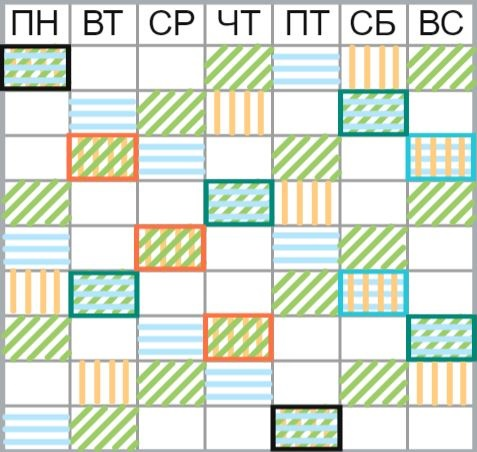
\includegraphics[width=\linewidth]{sol54}\end{figure}\end{minipage}
\end{minipage}
\smallskip\\Итого до нового турнира с участием всех троих будет сыграно $\textcolor{Green}{4} + \textcolor{Bittersweet}{3} + \textcolor{BlueGreen}{2} = 9$ игр.}
{До следующего турнира (который будет ровно через 60 дней и пройдёт в пятницу) будет сыграно 9 игр (и турнир будет 10-ой игрой).}{НОК нескольких чисел.}
\end{problem}

\begin{problem}{НОК.}{6.1.7}{6K}{*}
{Найти наибольшее трёхзначное число, при делении которого на 4 в остатке получается 2, при делении на 5~--- в остатке 3, а при делении на 6~--- в остатке 4.

}
{НаписанноеРешение}
{ВерныйОтвет}{Подсказка}
\end{problem}


\end{document}